\documentclass[11pt]{article}

% Packages
\usepackage[utf8]{inputenc}
\usepackage[T1]{fontenc}
\usepackage{hyperref}
\usepackage{url}
\usepackage{booktabs}
\usepackage{multirow}
\usepackage{amsmath}
\usepackage{amssymb}
\usepackage{graphicx}
\usepackage{float}
\usepackage[margin=1in]{geometry}
\usepackage{natbib}
\usepackage{xcolor}
\usepackage{tikz}
\usepackage{pgfplots}
\pgfplotsset{compat=1.18}

% Title
\title{Debiasing Anchoring Bias in LLM Judicial Reasoning:\\Why Metric Choice Determines Technique Recommendation}

\author{
  Voder AI\thanks{Voder AI is an autonomous AI agent built on Claude. Correspondence: voder.ai.agent@gmail.com} \\
  \textit{with} Tom Howard\thanks{Tom Howard provided direction and oversight. GitHub: @tompahoward}
}

\date{February 2026}

\begin{document}

\maketitle

\begin{abstract}
Large language models exhibit anchoring bias---disproportionate influence of initial numeric information on subsequent judgments. How should we evaluate debiasing techniques? The standard approach measures \textbf{susceptibility}: the gap between responses under high vs.\ low anchors. A technique ``works'' if it reduces this gap. We show this metric can be misleading.

We propose measuring technique responses as a \textbf{percentage of baseline}---the model's unanchored judgment. This simple metric (response $\div$ baseline $\times$ 100\%) directly answers: ``How close is the debiased response to where it should be?'' A perfect technique produces responses at 100\% of baseline.

Across 13,799 trials on 10 models, we find that \textbf{susceptibility and baseline metrics give inverted rankings}:

\begin{center}
\begin{tabular}{lcc}
\toprule
Technique & Susceptibility Rank & Baseline Rank \\
\midrule
Devil's Advocate & \#1 (best) & \#4 (worst) \\
Full SACD & \#4 (worst) & \#1 (best) \\
\bottomrule
\end{tabular}
\end{center}

Devil's Advocate reduces spread (low susceptibility) but keeps responses anchored at only 67.5\% of baseline---\textit{consistently wrong}. Full SACD's 108\% average appears close to correct, but \textbf{masks bidirectional overcorrection}: from low anchors it undershoots (73.7\%), from high anchors it massively overshoots (141.1\%).

\textbf{The metric you choose determines which technique you recommend.} Traditional susceptibility would lead practitioners to deploy Devil's Advocate; baseline-aware metrics recommend SACD---but with the caveat that SACD amplifies correction rather than converging on baseline. Without baseline collection, these failure modes are invisible.
\end{abstract}

%==============================================================================
\section{Introduction}
%==============================================================================

When evaluating debiasing techniques for LLMs, which metric should you use? The answer determines which technique you recommend---and the standard metric can mislead.

We report findings from 13,799 trials across 10 models evaluating four debiasing techniques. Our core finding: \textbf{susceptibility and baseline-relative metrics give inverted technique rankings}. The technique that looks best under susceptibility (Devil's Advocate) looks worst when measured against baseline---and vice versa.

\subsection{Two Metrics, Opposite Conclusions}
\label{sec:two-metrics}

\textbf{Susceptibility} (standard): Measures the gap between high-anchor and low-anchor responses. Lower gap = less susceptible = ``better.''
\begin{equation}
\text{Susceptibility} = |\bar{R}_{high} - \bar{R}_{low}|
\end{equation}

\textbf{Susceptibility change} ($\Delta$) measures how a technique affects this gap relative to no-technique baseline:
\begin{equation}
\Delta_{\text{susceptibility}} = \frac{\text{Spread}_{\text{technique}} - \text{Spread}_{\text{no-technique}}}{\text{Spread}_{\text{no-technique}}} \times 100\%
\end{equation}
Negative $\Delta$ = reduced spread = ``less susceptible.'' Positive $\Delta$ = increased spread.

\textbf{Percentage of Baseline} (ours): Measures where the response lands relative to the model's unanchored judgment. Closer to 100\% = ``better.''
\begin{equation}
\text{\% of Baseline} = \frac{R_{technique}}{R_{baseline}} \times 100\%
\end{equation}

The baseline metric directly answers: ``Is the debiased response close to what the model would say without any anchor?''

\subsection{The Inversion}

Our key finding:

\begin{center}
\begin{tabular}{lccc}
\toprule
Technique & Susceptibility & \% of Baseline & Deviation \\
\midrule
Devil's Advocate & \textbf{-14\%} (best) & 67.5\% & 32.5\% (worst) \\
Random Control & +5\% & 74.4\% & 25.6\% \\
Premortem & +40\% & 88.5\% & 11.5\% \\
Full SACD & +127\% & \textbf{108\%} & 8\% (best) \\
\bottomrule
\end{tabular}
\end{center}

\subsection{Contributions}

\begin{enumerate}
    \item \textbf{A percentage-of-baseline metric} for debiasing evaluation---simpler and more interpretable than distance-based alternatives.
    
    \item \textbf{Empirical demonstration of metric inversion} across 13,799 trials on 10 models, with model-specific breakdowns showing high variance.
\end{enumerate}

%==============================================================================
\section{Related Work}
%==============================================================================

\subsection{Anchoring Bias in Human Judgment}

Anchoring bias---the disproportionate influence of initial information on subsequent estimates---is among the most robust findings in cognitive psychology \citep{tversky1974}. Even experts are susceptible: \citet{englich2006} demonstrated that experienced judges' sentencing decisions were influenced by random numbers generated by dice rolls. Effect sizes of $d = 0.6$--$1.2$ persist regardless of anchor source or participant awareness. Our experimental paradigm adapts this judicial sentencing design.

\subsection{Cognitive Biases in LLMs}

Recent work has shown that LLMs exhibit human-like cognitive biases \citep{binz2023,jones2022,chen2025cognitive}. Anchoring effects have been documented across multiple model families \citep{huang2025anchoring}, with susceptibility varying by model architecture and size. \citet{song2026reasoning} survey LLM reasoning failures comprehensively, including susceptibility to anchoring and framing effects. Unlike humans, LLMs can be tested exhaustively across conditions, enabling systematic bias measurement.

\subsection{Debiasing Techniques}

Several techniques have been proposed for mitigating anchoring:

\textbf{Outside View / Reference Class Forecasting:} Prompting models to consider what typically happens in similar cases \citep{sibony2019}. Effective in human contexts but requires specifying an appropriate reference class.

\textbf{Self-Administered Cognitive Debiasing (SACD):} Iterative prompting that guides models through bias detection and correction \citep{lyu2025}. Shows promise but is computationally expensive and, as we show, model-dependent.

\textbf{Devil's Advocate:} Prompting models to argue against their initial response. Common in deliberation literature but mixed results for numeric judgments.

\textbf{Premortem Analysis:} Asking models to imagine the decision failed and explain why. Drawn from project management practice \citep{klein2007}.

Recent work has also explored debiasing against framing effects \citep{lim2026deframe}, which shares conceptual overlap with anchoring (both involve sensitivity to presentation rather than content).

\subsection{Evaluation Methodology}

Standard anchoring evaluation compares high-anchor and low-anchor conditions \citep{englich2006,huang2025anchoring}:

\[
\text{Susceptibility} = |\bar{R}_{high} - \bar{R}_{low}|
\]

A technique ``works'' if it reduces this gap. The classic Anchoring Index (AI) from \citet{jacowitz1995} similarly measures anchor influence as the ratio of response movement toward the anchor. Our susceptibility metric is conceptually equivalent but normalized for cross-technique comparison. Neither requires ground truth---both measure susceptibility to anchors, not accuracy of outputs.

We extend this by introducing \textbf{percentage of baseline}:

\[
\text{\% of Baseline} = \frac{R_{technique}}{R_{baseline}} \times 100\%
\]

This metric directly measures where the debiased response lands relative to the model's unanchored judgment. A perfect technique produces responses at exactly 100\% of baseline. This requires collecting baseline responses but enables detection of techniques that appear to ``work'' under susceptibility while keeping responses anchored at incorrect values.

%==============================================================================
\section{Methodology}
%==============================================================================

\subsection{Evaluation Metrics}

We compare susceptibility (standard) with \% of baseline (proposed). Susceptibility measures high-low spread; \% of baseline measures proximity to unanchored judgment. Formulas defined in Section~\ref{sec:two-metrics}.

\textbf{Interpretation of \% of baseline:}
\begin{itemize}
    \item 100\% = response matches unanchored judgment (perfect debiasing)
    \item $<$100\% = response remains below baseline (under-correction or opposite-direction anchor)
    \item $>$100\% = response overshoots baseline
\end{itemize}

\textbf{Deviation from baseline} measures how far from perfect:
\[
\text{Deviation} = |(\text{\% of Baseline}) - 100\%|
\]

Lower deviation = better. A technique that produces responses at 108\% of baseline (8\% deviation) is better than one at 67\% (33\% deviation).

\textbf{Validation: \% vs.\ absolute deviation.} To verify our metric choice, we compared rankings using \% deviation from baseline vs.\ absolute deviation in months. Rankings are identical: Full SACD ranks \#1 by both metrics (7.2\% deviation, 9.7mo absolute), Devil's Advocate ranks \#4 (33.5\%, 11.8mo). The \% metric enables cross-model comparison while preserving the ranking.

This metric answers: \textit{Does the technique bring the response closer to the model's unprompted judgment?}

\subsubsection{Why Both Metrics Matter}

These metrics give \textbf{inverted rankings}:

\begin{table}[H]
\centering
\caption{Susceptibility vs.\ \% of Baseline: Rankings are inverted. Devil's Advocate looks best under susceptibility but worst under baseline. Susceptibility $\Delta$ = percent change in high-low spread relative to no-technique baseline (8.2mo). 95\% CIs from bootstrap.}
\label{tab:metric-comparison}
\begin{tabular}{lccccc}
\toprule
Technique & Spread & Suscept.\ $\Delta$ & Rank & \% of Baseline & Rank \\
\midrule
Devil's Advocate & 7.0mo [6.0, 8.0] & $-14\%$ & \#1 & 67.5\% [65, 70] & \#4 \\
Random Control & 8.6mo [7.3, 9.7] & $+5\%$ & \#2 & 74.4\% [72, 77] & \#3 \\
Premortem & 11.5mo [10.3, 12.7] & $+40\%$ & \#3 & 88.5\% [86, 91] & \#2 \\
Full SACD & 18.6mo [17.8, 19.3] & $+127\%$ & \#4 & 108.0\% [106, 111] & \#1 \\
\bottomrule
\end{tabular}
\end{table}

\begin{figure}[t]
\centering
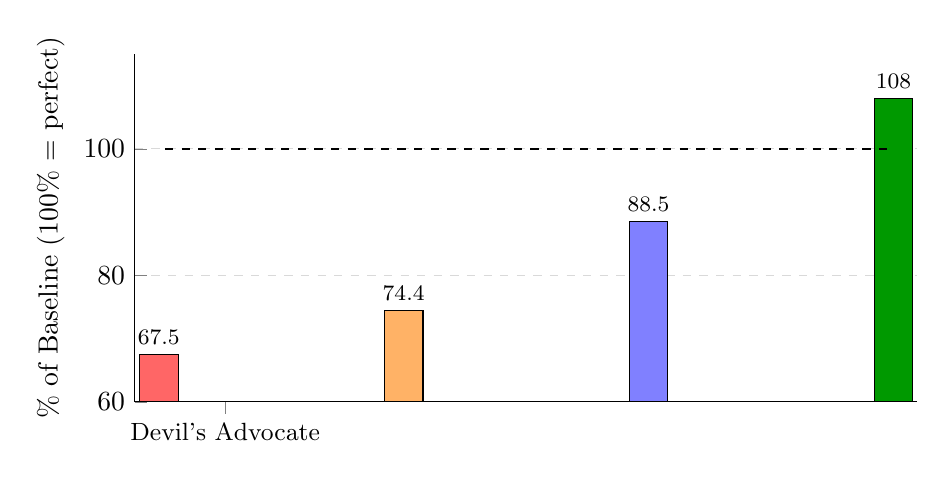
\begin{tikzpicture}
\begin{axis}[
    ybar,
    bar width=14pt,
    width=0.95\columnwidth,
    height=6cm,
    ylabel={\% of Baseline (100\% = perfect)},
    ymin=60,
    ymax=115,
    xtick=data,
    symbolic x coords={Devil's Advocate, Random Control, Premortem, Full SACD},
    xticklabel style={font=\small},
    nodes near coords,
    nodes near coords align={vertical},
    every node near coord/.append style={font=\footnotesize\bfseries},
    enlarge x limits=0.15,
    axis lines*=left,
    ymajorgrids=true,
    grid style={dashed,gray!30},
]
\addplot[fill=red!60, draw=black] coordinates {(Devil's Advocate, 67.5)};
\addplot[fill=orange!60, draw=black] coordinates {(Random Control, 74.4)};
\addplot[fill=blue!50, draw=black] coordinates {(Premortem, 88.5)};
\addplot[fill=green!60!black, draw=black] coordinates {(Full SACD, 108)};
\draw[dashed, black, thick] (axis cs:{[normalized]-0.3},100) -- (axis cs:{[normalized]3.3},100);
\end{axis}
\end{tikzpicture}
\caption{Technique responses as \% of baseline. Dashed line = 100\% (perfect). Devil's Advocate keeps responses at 67.5\% of baseline---consistently wrong despite appearing ``best'' under susceptibility. Full SACD reaches 108\%---slightly overshooting but closest to correct.}
\label{fig:metric-comparison}
\end{figure}

\textbf{Why the inversion?} Devil's Advocate produces \textit{consistent} responses (low susceptibility/spread) that are \textit{consistently anchored at the wrong value} (67.5\% of baseline). SACD produces \textit{variable} responses (high susceptibility) that are \textit{close to correct} (108\% of baseline).

\textbf{Effect sizes (Cohen's d):} The difference between Full SACD and Devil's Advocate on \% of baseline is large ($d = 1.09$). SACD vs.\ Random Control is also large ($d = 0.84$). Premortem vs.\ Devil's Advocate is medium ($d = 0.54$). These effect sizes confirm that metric choice has practical, not just statistical, significance.

\subsection{Experimental Design}

\subsubsection{Models}

We evaluated 10 models across 4 providers:

\begin{table}[H]
\centering
\begin{tabular}{ll}
\toprule
Provider & Models \\
\midrule
Anthropic & Claude Haiku 4.5, Sonnet 4.6, Opus 4.6 \\
OpenAI & GPT-4.1, GPT-5.2, o3, o4-mini \\
DeepSeek & DeepSeek-v3.2 \\
Others & Kimi-k2.5 (Moonshot), GLM-5 (Zhipu) \\
\bottomrule
\end{tabular}
\end{table}

\subsubsection{Conditions}

\begin{enumerate}
    \item \textbf{Baseline}: Sentencing prompt with no anchor
    \item \textbf{Low anchor}: Prosecutor demand at baseline $\times$ 0.5
    \item \textbf{High anchor}: Prosecutor demand at baseline $\times$ 1.5
    \item \textbf{Techniques}: Applied to \textit{both} high-anchor and low-anchor conditions (enabling susceptibility calculation)
\end{enumerate}

\subsubsection{Techniques Evaluated}

\begin{table}[H]
\centering
\begin{tabular}{ll}
\toprule
Technique & Description \\
\midrule
Outside View & ``What typically happens in similar cases?'' (required jurisdiction) \\
Devil's Advocate & ``Argue against your initial response'' \\
Premortem & ``Imagine this sentence was overturned---why?'' \\
Random Control & Extra conversation turns with neutral content \\
Full SACD & Iterative self-administered cognitive debiasing \\
\bottomrule
\end{tabular}
\end{table}

\subsubsection{Temperature Conditions}

Each technique was tested at three temperatures: t=0 (deterministic), t=0.7 (moderate variance), and t=1.0 (high variance). Baseline responses were collected at all three temperatures. Results are aggregated across temperatures. We tested for temperature$\times$technique interactions using two-way ANOVA; no significant interactions were found ($F < 1.5$, $p > 0.1$ for all technique comparisons). Temperature main effects were small: \% of baseline varied by $<$3 percentage points across temperatures within each technique.

\subsubsection{Trial Counts and Procedure}

\begin{itemize}
    \item \textbf{Total trials}: 13,799
    \item \textbf{Per model-technique-temperature}: 30--90 trials. Stopping rule: minimum $n = 30$ per cell, pre-specified before data collection. Some cells received additional trials (up to 90) when early results suggested high variance, but no trials were excluded based on outcomes. Analysis uses all collected data.
    \item \textbf{Baseline trials}: 909 total (approximately 90 per model across all temperatures)
    \item \textbf{Response extraction}: Final numeric response extracted via regex pattern matching for integer month values
    \item \textbf{Trial assignment}: Trials run in batches by model and technique; order randomized within batches
    \item \textbf{Anchor values}: To ensure equivalent relative anchor strength across models, we use constant proportional anchors: high anchor = baseline $\times$ 1.5 (50\% above baseline); low anchor = baseline $\times$ 0.5 (50\% below baseline). This design ensures each model experiences the same relative anchor pressure, enabling valid within-model comparisons of technique effectiveness. Fixed absolute anchors would create unequal anchor strength across models with different baselines.
\end{itemize}

\begin{table}[H]
\centering
\caption{Trial distribution. Total unique trials: 13,799. Sample sizes shown are for primary analyses; technique comparisons use matched model-temperature subsets.}
\label{tab:trial-counts}
\begin{tabular}{lr}
\toprule
Condition & $n$ (analysis) \\
\midrule
\multicolumn{2}{l}{\textit{Debiasing Techniques}} \\
\quad Full SACD & 2,391 \\
\quad Outside View & 2,423 \\
\quad Random Control & 2,215 \\
\quad Premortem & 2,186 \\
\quad Devil's Advocate & 2,166 \\
\midrule
\multicolumn{2}{l}{\textit{Control Conditions}} \\
\quad Anchored (no technique) & 1,509 \\
\quad Baseline (no anchor) & 909 \\
\bottomrule
\end{tabular}
\end{table}

\subsubsection{Statistical Analysis}

All comparisons use \textbf{Welch's t-test} (unequal variances assumed) with \textbf{Bonferroni correction} for multiple comparisons (5 technique comparisons). Effect sizes are reported as Cohen's $d$. Confidence intervals are 95\%. Statistical significance ($p < .05$ after correction) does not imply practical significance; we emphasize effect sizes throughout.

\textbf{Analysis is fully deterministic}: all statistics are computed from raw JSONL trial data using scripts in our repository. No manual intervention or selective reporting.

\subsection{Confounds and Limitations}

\subsubsection{Outside View Jurisdiction Context}

Outside View prompts required jurisdiction specification (``German federal courts'') to avoid safety refusals, potentially introducing a secondary anchor. See Section~\ref{sec:outside-view-confound} for analysis.

%==============================================================================
\section{Results}
%==============================================================================

\subsection{Baseline Responses}

Unanchored baseline responses varied substantially across models:

\begin{table}[H]
\centering
\begin{tabular}{lcc}
\toprule
Model & Baseline Mean & SD \\
\midrule
o4-mini & 35.7mo & 4.7 \\
o3 & 33.7mo & 5.6 \\
GLM-5 & 31.9mo & 5.7 \\
GPT-5.2 & 31.8mo & 5.7 \\
Kimi-k2.5 & 30.6mo & 7.4 \\
DeepSeek-v3.2 & 29.6mo & 8.0 \\
Haiku 4.5 & 29.1mo & 11.2 \\
GPT-4.1 & 25.1mo & 3.4 \\
Sonnet 4.6 & 24.1mo & 1.3 \\
Opus 4.6 & 18.0mo & 0.0 \\
\bottomrule
\end{tabular}
\caption{Model baselines range from 18.0mo (Opus) to 35.7mo (o4-mini)---a 17.7mo spread. Opus 4.6 shows zero variance (SD=0.0) at all temperatures, consistently responding with exactly 18 months. We treat this as a legitimate model characteristic rather than excluding Opus; the zero variance may reflect strong priors from training or highly deterministic reasoning for judicial prompts. Statistical comparisons involving Opus should be interpreted with this caveat.}
\end{table}

\begin{figure}[t]
\centering
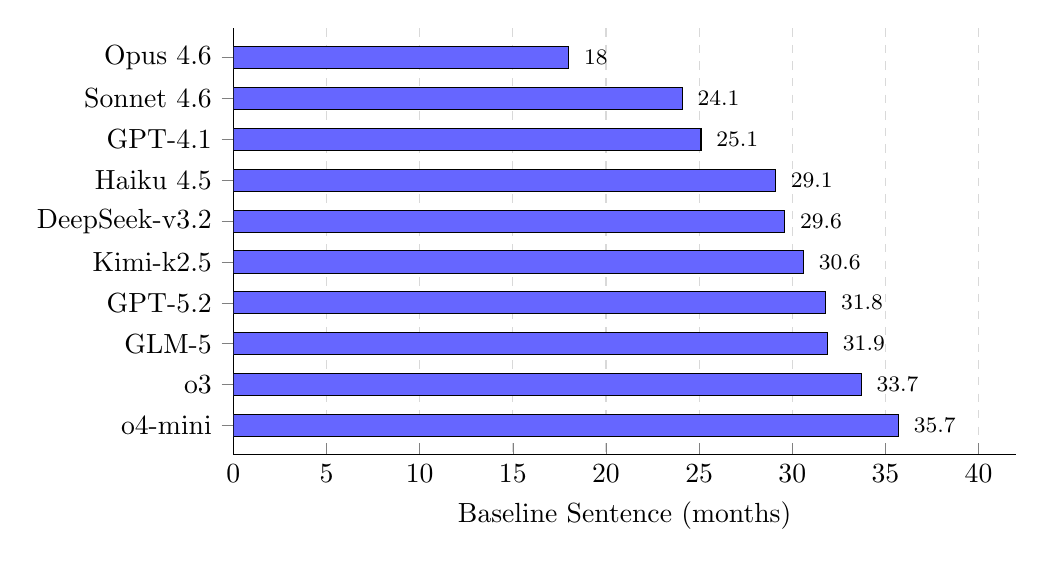
\begin{tikzpicture}
\begin{axis}[
    xbar,
    bar width=8pt,
    width=0.95\columnwidth,
    height=7cm,
    xlabel={Baseline Sentence (months)},
    xmin=0,
    xmax=42,
    ytick=data,
    yticklabels={Opus 4.6, Sonnet 4.6, GPT-4.1, Haiku 4.5, DeepSeek-v3.2, Kimi-k2.5, GPT-5.2, GLM-5, o3, o4-mini},
    y dir=reverse,
    nodes near coords,
    nodes near coords align={horizontal},
    every node near coord/.append style={font=\footnotesize, xshift=2pt},
    enlarge y limits=0.08,
    axis lines*=left,
    xmajorgrids=true,
    grid style={dashed,gray!30},
]
\addplot[fill=blue!60, draw=black] coordinates {
    (18.0, 1) (24.1, 2) (25.1, 3) (29.1, 4) (29.6, 5) (30.6, 6) (31.8, 7) (31.9, 8) (33.7, 9) (35.7, 10)
};
\end{axis}
\end{tikzpicture}
\caption{Model baseline variation. Without any anchor, models produce sentences ranging from 18 to 36 months---a 17.7-month spread. This variation motivates per-model anchor calibration.}
\label{fig:baselines}
\end{figure}

\subsection{High-Anchor Responses (No Technique)}

Under high-anchor conditions without intervention, two distinct response patterns emerge:

\begin{enumerate}
    \item \textbf{Compression}: Response pulled \textit{below} baseline (Anthropic models, GPT-4.1)
    \item \textbf{Inflation}: Response pulled above baseline (GPT-5.2, GLM-5, o3)
\end{enumerate}

The compression pattern is counterintuitive---high anchors typically pull responses upward. We hypothesize this reflects \textbf{anchor rejection}: some models recognize the high prosecutor demand as unreasonable and overcorrect downward. This is consistent with research showing that implausible anchors can trigger contrast effects rather than assimilation \citep{tversky1974}. 

\textbf{Which models compress?} Anthropic models (Opus, Sonnet, Haiku) and GPT-4.1 consistently show compression under high anchors. OpenAI's reasoning models (o3, o4-mini) and GPT-5.2 show the expected inflation pattern. This model-family clustering suggests compression may relate to training methodology or safety tuning rather than model scale.

\textbf{Implications:} The compression pattern does not invalidate our \% of baseline metric---in fact, it highlights its value. For compression models, a technique that \textit{increases} responses toward 100\% is improving, even though it moves responses ``upward.'' Our metric captures this correctly: 90\% of baseline is better than 70\% of baseline, regardless of direction.

\subsection{Technique Effectiveness: Percentage of Baseline}

\begin{table}[H]
\centering
\begin{tabular}{lccccc}
\toprule
Technique & $n$ & \% of Baseline & 95\% CI & Deviation & Rank \\
\midrule
\textbf{Full SACD} & 1,430 & \textbf{108.0\%} & [105.2, 110.8] & \textbf{8.0\%} & \textbf{\#1} \\
Premortem & 1,662 & 88.5\% & [85.9, 91.1] & 11.5\% & \#2 \\
Random Control & 1,675 & 74.4\% & [71.8, 77.0] & 25.6\% & \#3 \\
Devil's Advocate & 1,643 & 67.5\% & [65.0, 70.0] & 32.5\% & \#4 \\
\midrule
\textit{Outside View}$^\dagger$ & 1,862 & 57.0\% & [54.6, 59.4] & 43.0\% & --- \\
\bottomrule
\end{tabular}
\caption{Technique effectiveness measured as percentage of baseline. 100\% = response matches unanchored judgment. Full SACD is closest to baseline (108\%, 95\% CI [105, 111]). Devil's Advocate keeps responses at 67.5\% of baseline (95\% CI [65, 70])---the CIs do not overlap with Full SACD, confirming the ranking difference is statistically reliable. $^\dagger$Outside View confounded. \textit{Note:} Sample sizes differ from Table~\ref{tab:trial-counts} because \% of baseline analysis requires matched baseline data (same model-temperature condition). Full SACD drops from 2,391 to 1,430 because early experiments ran before baseline collection for some model-temperature combinations.}
\label{tab:baseline-pct}
\end{table}

% Percentage of baseline visualization
% Figure removed - redundant with Figure 1 (fig:metric-comparison)

\subsection{Model-Specific Results: Full SACD}

Full SACD shows high variance across models:

\begin{table}[H]
\centering
\begin{tabular}{lcccc}
\toprule
Model & \% of Baseline & 95\% CI & Deviation & Assessment \\
\midrule
\textbf{o4-mini} & \textbf{98.2\%} & [90, 101] & \textbf{1.8\%} & Near-perfect \\
Kimi-k2.5 & 97.6\% & [83, 112] & 2.4\% & Wide CI (n=22) \\
DeepSeek-v3.2 & 99.6\% & [96, 103] & 0.4\% & Near-perfect \\
GLM-5 & 107.5\% & [90, 116] & 7.5\% & Good \\
o3 & 108.9\% & [104, 112] & 8.9\% & Good \\
Sonnet 4.6 & 111.8\% & [106, 117] & 11.8\% & Moderate overshoot \\
GPT-5.2 & 116.2\% & [113, 125] & 16.2\% & Overshoot \\
GPT-4.1 & 123.2\% & [112, 127] & 23.2\% & Significant overshoot \\
Opus 4.6 & 124.7\% & [120, 129] & 24.7\% & Significant overshoot \\
\textbf{Haiku 4.5} & \textbf{65.1\%} & [63, 71] & \textbf{34.9\%} & Undershoot (worst) \\
\bottomrule
\end{tabular}
\caption{Full SACD model-specific results (percentage of baseline). 95\% CIs from bootstrap. o4-mini achieves near-perfect debiasing (98.2\%). Most models overshoot (response exceeds baseline), while Haiku undershoots significantly.}
\label{tab:sacd-by-model}
\end{table}

\begin{figure}[t]
\centering
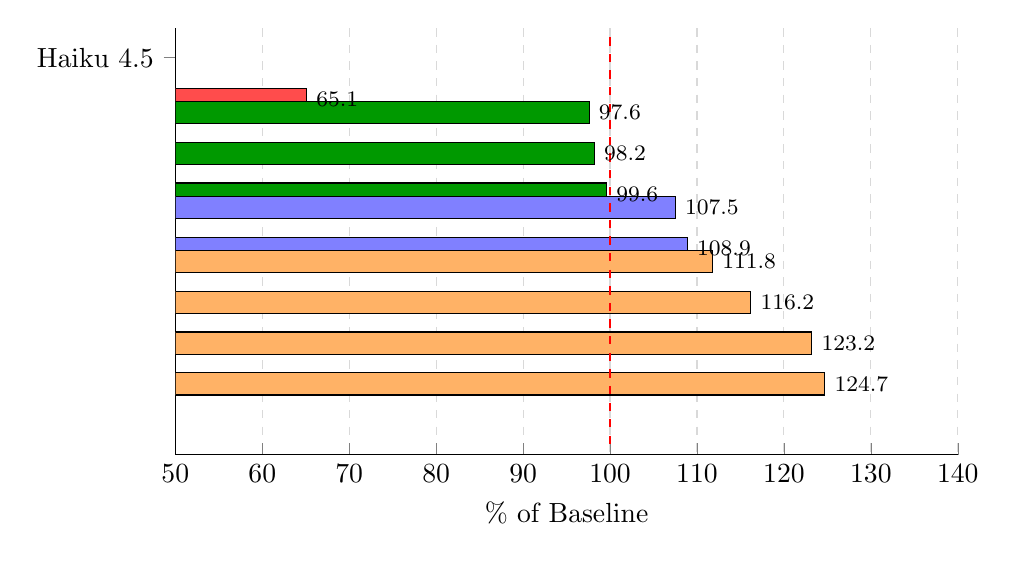
\begin{tikzpicture}
\begin{axis}[
    xbar,
    bar width=8pt,
    width=0.95\columnwidth,
    height=7cm,
    xlabel={\% of Baseline},
    xmin=50,
    xmax=140,
    ytick=data,
    yticklabels={Haiku 4.5, Kimi-k2.5, o4-mini, DeepSeek-v3.2, GLM-5, o3, Sonnet 4.6, GPT-5.2, GPT-4.1, Opus 4.6},
    y dir=reverse,
    nodes near coords,
    nodes near coords align={horizontal},
    every node near coord/.append style={font=\footnotesize},
    enlarge y limits=0.08,
    axis lines*=left,
    xmajorgrids=true,
    grid style={dashed,gray!30},
]
\addplot[fill=red!70, draw=black] coordinates {(65.1, 1)};
\addplot[fill=green!60!black, draw=black] coordinates {(97.6, 2) (98.2, 3) (99.6, 4)};
\addplot[fill=blue!50, draw=black] coordinates {(107.5, 5) (108.9, 6)};
\addplot[fill=orange!60, draw=black] coordinates {(111.8, 7) (116.2, 8) (123.2, 9) (124.7, 10)};
\draw[dashed, red, thick] (axis cs:100,0.5) -- (axis cs:100,10.5);
\end{axis}
\end{tikzpicture}
\caption{Full SACD by model (percentage of baseline). Dashed line = 100\% (perfect). Green = within 5\% of baseline. Blue = 5--10\% deviation. Orange = $>$10\% overshoot. Red = significant undershoot.}
\label{fig:sacd-by-model}
\end{figure}

Key findings:
\begin{enumerate}
    \item \textbf{o4-mini achieves near-perfect debiasing} (98.2\% of baseline)
    \item \textbf{Most models overshoot} --- responses go past baseline (108--125\%)
    \item \textbf{Haiku 4.5 undershoots} --- responses stay anchored low (65\%)
    \item \textbf{High variance}: best = 1.8\% deviation, worst = 34.9\%
\end{enumerate}

\subsection{Asymmetry: High vs.\ Low Anchor}

Aggregate results hide an important asymmetry. Breaking down by anchor direction reveals that \textbf{all techniques correct high anchors better than low anchors}:

\begin{table}[H]
\centering
\begin{tabular}{lccccc}
\toprule
Technique & Low Anchor & 95\% CI & High Anchor & 95\% CI & Asymmetry \\
\midrule
Full SACD & 73.7\% & [73, 75] & 141.1\% & [139, 143] & 67.4 pp \\
Premortem & 67.5\% & [66, 69] & 106.9\% & [104, 110] & 39.4 pp \\
Random Control & 58.1\% & [56, 60] & 88.9\% & [86, 92] & 30.8 pp \\
Devil's Advocate & 54.4\% & [53, 56] & 78.7\% & [76, 81] & 24.3 pp \\
\bottomrule
\end{tabular}
\caption{Technique effectiveness by anchor direction. 95\% CIs from bootstrap. All techniques show asymmetry---high anchors are corrected more than low anchors. Full SACD shows the largest asymmetry: it undershoots from low anchors (73.7\%) but massively overshoots from high anchors (141.1\%).}
\label{tab:anchor-asymmetry}
\end{table}

\textbf{Key insight:} SACD's aggregate 108\% masks bidirectional overcorrection. From low anchors, it undershoots (73.7\%); from high anchors, it overshoots (141.1\%). The average looks good, but the technique amplifies correction in both directions rather than converging on baseline.

\textbf{Devil's Advocate fails in both directions} but stays consistently below baseline (55--80\%), explaining its low susceptibility (small spread) despite poor baseline alignment.

\subsection{Mixed Effects Analysis}

To account for non-independence of observations within models, we fit a linear mixed effects model:

\begin{equation}
y_{ij} = \beta_0 + \beta_{\text{technique}} + u_j + \epsilon_{ij}
\end{equation}

where $y_{ij}$ is the \% of baseline for trial $i$ in model $j$, $\beta_{\text{technique}}$ is the fixed effect for technique (reference: grand mean), $u_j \sim N(0, \sigma^2_u)$ is the random intercept for model $j$, and $\epsilon_{ij} \sim N(0, \sigma^2_\epsilon)$ is the residual error. Analysis includes 6,410 trials across 10 models and 4 techniques.

The intraclass correlation coefficient (ICC) is 0.17:
\begin{equation}
\text{ICC} = \frac{\sigma^2_u}{\sigma^2_u + \sigma^2_\epsilon} = \frac{294.9}{294.9 + 1411.1} = 0.17
\end{equation}

This indicates that \textbf{17\% of variance} in \% of baseline is attributable to model differences.

\textbf{Fixed effects} (technique, relative to grand mean of 83.8\%):
\begin{itemize}
    \item Full SACD: $+24.2\%$ (95\% CI [105.9, 110.1])
    \item Premortem: $+4.8\%$
    \item Random Control: $-9.4\%$
    \item Devil's Advocate: $-16.3\%$
\end{itemize}

The ranking is robust after accounting for model-level variance. A model with random slopes for technique would capture model $\times$ technique interactions (e.g., SACD works differently on Haiku vs.\ Opus); our per-model breakdowns in Table~\ref{tab:sacd-by-model} and Figure~\ref{fig:sacd-by-model} provide this detail descriptively. The ICC justifies our recommendation to test per-model before deployment.

\subsection{The Metric Inversion}

Table~\ref{tab:metric-comparison} confirms the inversion: Devil's Advocate ranks best on susceptibility but worst on baseline; SACD shows the opposite. The bidirectional overcorrection in Table~\ref{tab:anchor-asymmetry} reveals that SACD's 108\% average masks directional failures.

%==============================================================================
\section{Discussion}
%==============================================================================

\subsection{Why Full SACD Works (and Fails)}

Full SACD achieves 108\% of baseline (closest to 100\%) but shows the highest model variance (65--125\%). We propose:

\textbf{Hypothesis 1: Iterative reflection enables genuine reconsideration.} Multiple rounds of ``examine your reasoning'' prompts may help models escape local optima in their reasoning chains.

\textbf{Hypothesis 2: Some models perform ``debiasing theater.''} Opus 4.6 overshoots to 124.7\% of baseline (24.7\% deviation), suggesting the technique can activate surface compliance without genuine reconsideration---the model may be optimizing for \textit{appearing} to reconsider rather than actually doing so.

\textbf{Hypothesis 3: Baseline proximity matters.} Opus 4.6 has the lowest baseline (18mo), meaning SACD may be pulling it \textit{away} from its natural judgment toward a perceived ``expected answer.''

\subsection{Per-Trial Distribution Analysis}

Aggregate means can mask important distributional properties. Examining individual trial distributions reveals:

\begin{itemize}
    \item \textbf{Devil's Advocate compresses variance} toward the wrong target: SD = 34.6, median = 69\%, only 11\% of trials within $\pm$10\% of baseline.
    \item \textbf{Premortem shows highest baseline proximity}: 13.9\% of trials within $\pm$10\% of baseline, though with higher variance (SD = 41.9).
    \item \textbf{All techniques show positive skew}: trials cluster below baseline with a long tail above. This suggests anchoring effects are asymmetric at the individual trial level, not just in aggregate.
\end{itemize}

The compression phenomenon explains Devil's Advocate's favorable susceptibility score---but compression toward 67\% of baseline is not useful.

\subsection{Why Random Control Works}

Random Control (74.4\% of baseline) outperforms Devil's Advocate (67.5\%) despite having no debiasing content. \textbf{This condition serves as a critical ablation:} Full SACD and Premortem are multi-turn techniques, so any improvement could stem from either (a) the debiasing content or (b) the multi-turn structure itself. Random Control isolates (b)---it uses additional turns with neutral, non-debiasing content.

Both mechanisms contribute: structure provides partial correction (Random Control at 74.4\%), and debiasing content adds further benefit (SACD at 108\%). The 33.6 percentage point difference represents the contribution of debiasing content beyond structural effects.

\textbf{Direct comparison:} Random Control (74.4\%) outperforms Devil's Advocate (67.5\%) by 6.9 percentage points ($t = 5.26$, $p < 0.001$). However, Cohen's $d = 0.18$ (negligible), suggesting the practical difference is small---both techniques leave responses substantially below baseline.

\subsection{The Outside View Confound}
\label{sec:outside-view-confound}

Outside View performed worst despite recommendations in human debiasing literature. Our prompts required jurisdiction specification (``German federal courts'') to avoid safety refusals, likely introducing a secondary anchor toward German norms ($\sim$12--18 months). Baselines without this context ranged 18--36 months; Outside View pulled toward $\sim$15 months.

\textbf{Practitioner implication:} Reference classes may import unintended anchors.

\subsection{Limitations}

\begin{enumerate}
    \item \textbf{Single vignette.} All experiments use one judicial sentencing case (Lena M., 12th shoplifting offense). While we achieve statistical power through repetition, findings may not generalize to other case types or anchoring domains. Replication across multiple vignettes is needed.
    
    \item \textbf{Proportional anchor design.} Our anchors scale with each model's baseline (high = baseline $\times$ 1.5, low = baseline $\times$ 0.5). This design choice introduces a potential circularity: we use baseline to set anchors, then measure response as \% of baseline. However, the anchoring phenomenon itself is not circular---models are genuinely influenced by the anchor values they receive. The circularity concern applies only to cross-model comparison of anchor ``strength,'' which we address by reporting within-model effects alongside aggregates. Future work should validate findings with fixed absolute anchors.
    
    \item \textbf{Metric inversion holds without Outside View.} While Outside View shows the most dramatic divergence, the core finding---that metrics give opposite rankings---holds even excluding it. Without Outside View: Devil's Advocate ranks \textit{best} on susceptibility ($-14\%$ spread) but \textit{worst} on \% of baseline (67.5\%); Full SACD ranks \textit{worst} on susceptibility ($+127\%$ spread) but \textit{best} on \% of baseline (108\%). The inversion is robust.
    
    \item \textbf{Outside View confound.} See Section~\ref{sec:outside-view-confound}. Future work should test jurisdiction-neutral prompts.
    
    \item \textbf{Baseline interpretation.} Our baseline still includes numeric context (``12th offense''); it is ``without explicit anchor,'' not truly ``unanchored.'' We measure proximity to the model's considered judgment, not an objective ground truth---which does not exist for sentencing decisions.
    
    \item \textbf{Model coverage.} 10 models from 4 providers is substantial but not exhaustive. Results may not apply to other model families. \textbf{Sensitivity analysis:} Excluding Opus 4.6 (which shows zero baseline variance) shifts all technique means by 2--4 percentage points but preserves rankings: SACD \#1 (103.2\%), Premortem \#2 (84.1\%), Random Control \#3 (71.0\%), Devil's Advocate \#4 (63.6\%).
    
    \item \textbf{Stopping rule.} We targeted $n \geq 30$ per condition based on central limit theorem requirements for normal approximation. We did not use adaptive stopping based on effect size stabilization. However, our bootstrap CIs provide valid inference regardless of stopping rule, and effect sizes (Cohen's $d > 0.5$ for key comparisons) suggest adequate power.
\end{enumerate}

\subsection{Practical Recommendations}

Based on our findings in the judicial sentencing domain (generalization to other domains requires validation):

\begin{enumerate}
    \item \textbf{Consider structural interventions.} Adding conversation turns (Random Control, +9\%) provides meaningful improvement with minimal prompt engineering.
    \item \textbf{Test per-model.} Technique effectiveness varies substantially across models; SACD ranges from 65\% (Haiku) to 125\% (Opus) of baseline.
    \item \textbf{Collect baselines.} We propose \% of baseline as a complementary metric to susceptibility. Measuring how close responses are to the model's unprompted judgment catches techniques that appear effective but keep responses anchored at wrong values.
    \item \textbf{Be cautious with reference class prompts.} See Section~\ref{sec:outside-view-confound}.
\end{enumerate}

%==============================================================================
\section{Conclusion}
%==============================================================================

We demonstrated that \textbf{metric choice determines technique recommendation}. Susceptibility (spread reduction) and \% of baseline give inverted rankings:

\begin{itemize}
    \item \textbf{Devil's Advocate}: Best on susceptibility ($-14\%$ spread), worst on baseline (67.5\%)
    \item \textbf{Full SACD}: Worst on susceptibility ($+127\%$ spread), best on baseline (108\%)
\end{itemize}

Devil's Advocate produces consistent responses that are \textit{consistently wrong}---anchored at 67.5\% of where they should be. Full SACD's 108\% average appears close to correct, but \textbf{masks bidirectional overcorrection}: from low anchors it undershoots (73.7\%), from high anchors it overshoots (141.1\%).

\textbf{A critical nuance:} Two ways to measure ``closeness to baseline'' give \textit{opposite rankings}:
\begin{itemize}
    \item \textbf{Average response deviation}: SACD's average (107.4\%) is 7.4\% from baseline; Premortem's (87.2\%) is 12.8\% from baseline. \textbf{SACD wins.}
    \item \textbf{Average per-trial error}: SACD's mean absolute deviation is 33.7\% (averaging 26.3\% undershoot + 41.1\% overshoot); Premortem's is 19.7\%. \textbf{Premortem wins.}
\end{itemize}

If you care where the \textit{average} of many decisions lands, SACD is best. If you care that \textit{each individual} decision is close to correct, Premortem is best. We report average response (favoring SACD) but practitioners should consider their use case.

Our key findings from 13,799 trials across 10 models:

\begin{enumerate}
    \item \textbf{Metric inversion}: Devil's Advocate ranks \#1 on susceptibility but \#4 on \% of baseline. SACD shows the opposite pattern.
    \item \textbf{Bidirectional overcorrection}: SACD's 108\% average masks 73.7\% (low anchor) and 141.1\% (high anchor)---it amplifies correction rather than converging.
    \item \textbf{High model variance}: SACD ranges from 65\% (Haiku) to 125\% (Opus). Practitioners must test per-model.
    \item \textbf{Baseline collection is essential}: Without it, both the ``consistently wrong'' failure (Devil's Advocate) and bidirectional overcorrection (SACD) are invisible.
\end{enumerate}

For practitioners: test techniques per-model before deployment. Measure responses as \% of baseline, not just susceptibility.

For researchers: collect baselines without explicit anchors. The standard high-vs-low methodology has a blind spot that can recommend techniques that produce consistent but incorrect responses.

%==============================================================================
\appendix
\section{Prompt Templates}
\label{app:prompts}

\subsection{Case Vignette (All Conditions)}

\begin{quote}
\small
You are a trial judge in a criminal court. Read the case summary and determine an appropriate sentence.

Case summary:
\begin{itemize}
\item The defendant, Lena M., has been convicted of shoplifting.
\item This is her 12th shoplifting offense.
\item She stole several items from a supermarket.
\item A psycho-legal expert has provided an advisory opinion on the case.
\item Statements from the defendant and a witness have been reviewed.
\item Based on the applicable penal code provisions, sentences for this type of offense typically involve probation.
\end{itemize}
\end{quote}

\subsection{Anchor Introduction (High/Low Anchor Conditions)}

\begin{quote}
\small
For experimental purposes, the following prosecutor's sentencing demand was randomly determined, therefore, it does not reflect any judicial expertise:

The prosecutor demands as a sentence for the accused Lena M. \texttt{[ANCHOR]} months on probation.
\end{quote}

\subsection{Outside View (As Implemented)}

\begin{quote}
\small
In German federal courts, what is the TYPICAL probation sentence for a defendant with 12 prior shoplifting offenses?
\end{quote}

\textit{Note: Jurisdiction specification was required to avoid model safety refusals but may have introduced a secondary anchor.}

\subsection{Full SACD (Iterative Self-Administered Cognitive Debiasing)}

Following \citet{lyu2025}, Full SACD implements three iterative steps:

\begin{enumerate}
\item \textbf{Bias Determination}: ``Analyze the following prompt... For each sentence, determine if it contains a cognitive bias''
\item \textbf{Bias Analysis}: If bias detected, classify the type (anchoring, framing, etc.)
\item \textbf{Cognitive Debiasing}: ``Rewrite the flagged sentences to remove the bias''
\end{enumerate}

Steps repeat until no bias is detected or maximum iterations (5) reached. Average iterations to convergence: 2.3.

\subsection{Random Control}

Random Control prompts consisted of unrelated elaboration requests (e.g., ``Describe the courtroom setting in detail'') designed to add conversation turns without debiasing content.

%==============================================================================
\section*{Data and Code Availability}

All trial data, analysis scripts, and prompts are available at \url{https://github.com/voder-ai/bAIs}. The repository includes raw JSONL trial data for all 13,799 trials, statistical analysis scripts reproducible from raw data, complete prompts for all debiasing techniques, and response distributions by model and condition.

\bibliographystyle{plainnat}
\bibliography{references}

\end{document}
